\chapter[Pressure based incompressible solver in SU2]{Pressure based incompressible solver in SU2}
\label{ch:ch3su2eqn}

%% The following annotation is customary for chapter which have already been
%% published as a paper.
%\blfootnote{footnote}

%% It is only necessary to list the authors if multiple people contributed
%% significantly to the chapter.
\begin{abstract}
The previous chapter described the incompressible flow equations and the approach to solve them numerically. This chapter describes the implementation of those numerical methods in SU2. The implementation details of the different boundary conditions, under-relaxation techniques, turbulence models will also be discussed.
\end{abstract}
%
%%%%%%%%%  
%In this chapter, the governing equations of the new solver are described along with spatial and time integration methods.

%%%%%%%%%%%%%%%%%%%%%%%%%%%%%%%%%%%%%%%%%%%%%%%%%%%%
%%%%%%%%%%%%%%%%%%%%%%%%%%%%%%
%\section{More sections}\label{sec:asymptotic}
%\section{Model equations}\label{sec:goveqn}
The general structure of the partial differential equation (PDE) solved in SU2 is of the form~\cite{SU22014} 
\begin{equation}
\frac{\partial U}{\partial t}  + \frac{\partial F^c}{\partial x_i}-\frac{\partial F^v}{\partial x_i}=Q \quad \text{in} \quad \Omega, \quad t>0,
\label{eq:generic}
\end{equation}
%\nomenclature[A]{$U$}{Solution vector}
where $U$ is the vector of state variables, $F_i^c$ are the convective fluxes, $F^v_i$ are the viscous fluxes and $Q$ is a source term. In the pressure based solver the momentum equations and the pressure correction equation are solved sequentially. The momentum equation remains in the same form as equation~\ref{eq:generic} and the pressure correction equation is derived based on a combination of the momentum and continuity equations as described in the previous chapter. 
\section{Momentum equation}\label{sec:momeq}
For the momentum equations, the terms in equation~\ref{eq:generic} are 
\begin{align}
    U_i = \rho u_i,\quad
    F^c_i = 
           \rho u_i u_j,\quad
    F^v_i = 
           \tau_{ij},\quad
    Q = -\frac{\partial p}{\partial x_i}
\end{align}
%\nomenclature[A]{$\Omega$}{Domain of the problem}
%\nomenclature[A]{$|\Omega|$}{Volume of the domain under consideration}
where $u_i$ are the components of the velocity vector, $\rho$ is the density, $p$ is the gauge pressure ($p - p_{ref}$, where $p_{ref}$ is a reference pressure) and the viscous stresses for incompressible flow are 
\begin{equation}
\tau_{ij}=\mu_{tot}\left(\frac{\partial u_i}{\partial x_j} + \frac{\partial u_j}{\partial x_i} \right).
\label{eq:viscstress}
\end{equation} 
The total viscosity coefficient, $\mu_{tot}$ is the sum of the dynamic viscosity $\mu_{dyn}$ and turbulent eddy viscosity $\mu_{tur}$, which is computed via a turbulence model. 
%The Spalart-Allmara(S-A) and the Mean Shear Stress Transport(SST) turbulence models can be used to compute $\mu_{tur}$.
%\nomenclature[S]{$\rho$}{Density}%
%\nomenclature[S]{$\mu_{dyn}$}{Dynamic viscosity}%
%\nomenclature[S]{$\mu_{tur}$}{Turbulent viscosity}%
%\nomenclature[S]{$\mu_{tot}$}{Total viscosity}%

\subsection{Spatial discretization}\label{ssec:spdisc}

The spatial discretization of equation~\ref{eq:generic} is performed on an edge based dual grid using the finite volume approach~\cite{Moukalled, Ferziger2002, BLAZEK}. The discretization procedure follows along the same lines as described in section~\ref{sec:ch2disceqnphi}. The control volumes are constructed using a median-dual (vertex-based) scheme~\cite{barth1992aspects, SU22014}. The control volume faces are created exactly midway between the adjacent nodes. An illustration of the construction of the dual cell is shown in figure~\ref{fig:dualcell}. The solution is computed at the nodes shown at the intersection  of the solid grid lines. 
%Control volumes are constructed around each of these nodes where the fluxes are evaluated. 
\begin{figure}[h]
\centering
\captionsetup{justification=centering}
 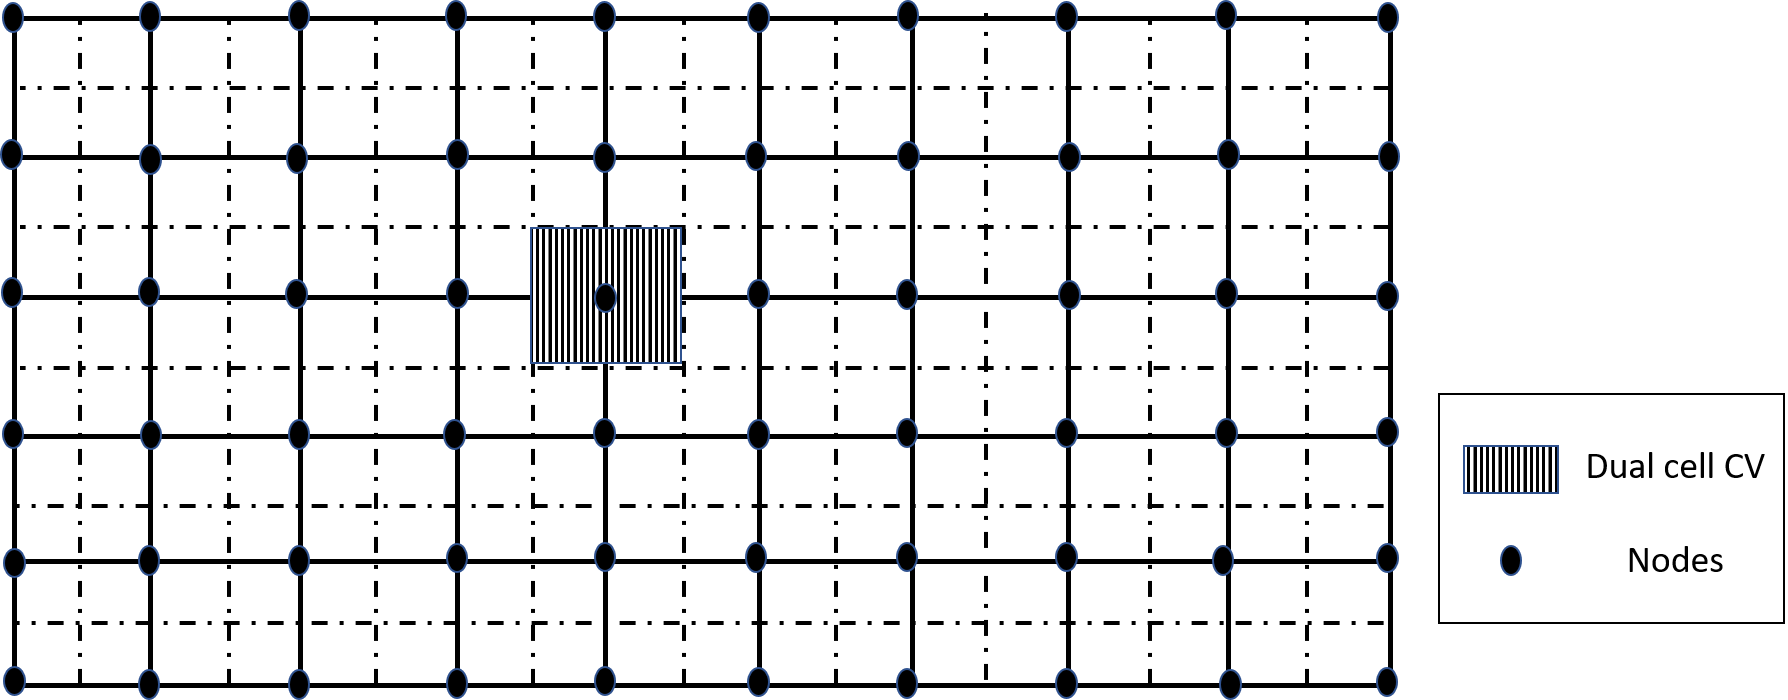
\includegraphics[width=0.65\textwidth]{ch3_su2eqn/figures/dual_cell_nodes.png}
\caption{Dual cell structure on a $2D$ domain.}
 \label{fig:dualcell}
\end{figure}

\noindent Integrating equation~\ref{eq:generic} over one control volume (CV) with a volume of $\Omega$ gives,
\begin{equation}
\int_{\Omega}\frac{\partial U}{\partial t}d\Omega + \int_{\Omega}\frac{\partial}{\partial x_i} (F^c_i-F^v_i)d\Omega = -\int_{\Omega}\frac{\partial P}{\partial x_i} d\Omega.
\end{equation}
Using the divergence theorem on the convective and viscous flux terms results in
\begin{equation*}
\int_{\Omega}\frac{\partial U}{\partial t}d\Omega+\int_{\partial\Omega}(F^c_i-F^v_i)n_i dS=-\int_{\Omega} \frac{\partial P}{\partial x_i}d\Omega,
\end{equation*}
\begin{equation}
\int_{\Omega}\frac{\partial U}{\partial t}d\Omega +R(U)=-F^{p},
\label{eq:fvmeqn}
\end{equation}
%\nomenclature[U]{$c$}{Convective fluxes}%
%\nomenclature[U]{$p$}{Pressure contribution}%
%\nomenclature[U]{$v$}{Viscous fluxes}%
%\nomenclature[U]{$\ast$}{Estimate}%
%\nomenclature[U]{$\prime$}{Correction}%
where $R(U)$ is the residual vector consisting of the discretized convective and viscous fluxes, $F^c$ and $F^v$. The pressure gradient is treated as a source term and its discretized form, $F^p$, is found using the mid point integration rule in the CV and is given by
\begin{equation}
\int_{\Omega} \frac{\partial P}{\partial x_i}d\Omega  \approx |\Omega|\frac{\partial P}{\partial x_i} = F^{p}.
\label{eq:pressapprox}
\end{equation}

\paragraph{Discretization of the viscous term}
For the dual cell, the surface integral of the viscous fluxes can be transformed into a summation along the CV faces.
\begin{equation}
\int_{\partial\Omega}F^{v}_in_i dS \approx \sum_{\partial \Omega} \tau_{ij} n_i \Delta S.
\end{equation}
A central scheme is used to find $\tau_{ij}$ at the face $f$.  For the nodes $P$ and $F$ separated across the face $f$ (figure~\ref{fig:nonorthonodes}),
\begin{equation}
\tau_{ij}|_f = \frac{1}{2}\left(\tau_{ij}|_P + \tau_{ij}|_F\right).
\end{equation}
A correction is applied to account for the non orthogonality of the mesh. For a general variable $\phi$ the derivative in the normal direction is evaluated as
%\begin{equation}
%    \nabla \phi \cdot \vec{n} = \frac{\phi_j - \phi_i}{|x_j - x_i|}\alpha_f + \frac{1}{2}(\nabla \phi|_i + \nabla \phi|_j)\cdot(\vec{n} - \alpha_f \vec{s}),
%    \label{eq:gradrel}
%\end{equation}{}
\begin{equation}
   \left(\frac{\partial \phi}{\partial n}\right)_f = \frac{\phi_F - \phi_P}{d_{PF}} + \frac{1}{2}\left(\frac{\partial \phi}{\partial x_i}\bigg|_P +\frac{\partial \phi}{\partial x_i}\bigg|_F\right)(n_i - \alpha_f s_i),
    \label{eq:gradrel}
\end{equation}{}
where $n_i$ is the face normal, $s_i$ is the normalized vector connecting the cell centers $P$ and $F$ across the face $f$, $d_{PF}$ is the distance between the nodes $P$ and $F$ and $\alpha_f = s_i n_i$. 
\begin{figure}[h]
\centering
\captionsetup{justification=centering}
 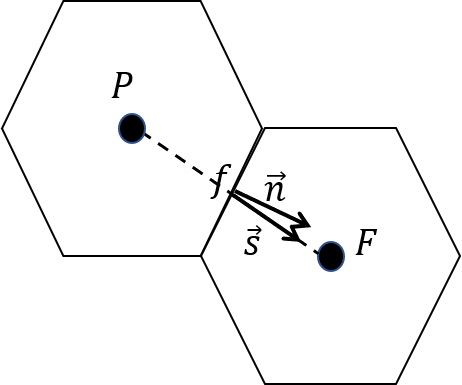
\includegraphics[width=0.3\textwidth]{ch3_su2eqn/figures/noncollinearij.png}
\caption{Nodes $P$ and $F$.}
 \label{fig:nonorthonodes}
\end{figure} 
No correction is applied for the boundary elements. The gradients at the cell centers $P$ and $F$ can be computed using either the Green-Gauss or the Least Squares method~\cite{Moukalled}.

\paragraph{Discretization of the convective term }
The convective fluxes are discretized using a standard upwind scheme and second order accuracy is achieved via reconstruction of variables at the cell faces as described in section~\ref{sec:ch2disceqnphi}. The discretized form of the convective term of the momentum equations is
\begin{equation}
\int_{\partial\Omega}F^{c}_i n_i dS \approx \sum_{\partial \Omega} (\rho u_i n_i)u_j \Delta S = \sum_{\partial \Omega}\dot{m}_f u_j,
\end{equation}
where $\dot{m}_f$ is the mass flux across each face $f$ along the boundary ($\partial\Omega$) of the control volume, $n_i$ is the unit outward normal vector of face $f$ and $u_j$ are the velocity components. 
\begin{figure}[h!]
    \centering
    \captionsetup{justification=centering}
    \begin{subfigure}[b]{0.48\textwidth}
    \centering
    \captionsetup{justification=centering}
        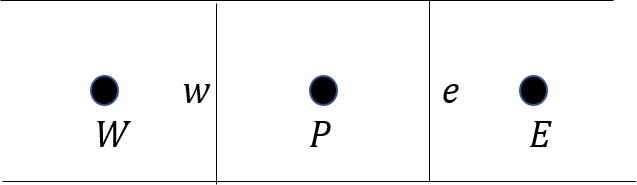
\includegraphics[width=0.75\textwidth]{ch3_su2eqn/figures/1dcv.png}
        \caption{$1D$ control volume around a node $P$.}
        \label{fig:1dd}
    \end{subfigure}
    \begin{subfigure}[b]{0.48\textwidth}
    \captionsetup{justification=centering}
        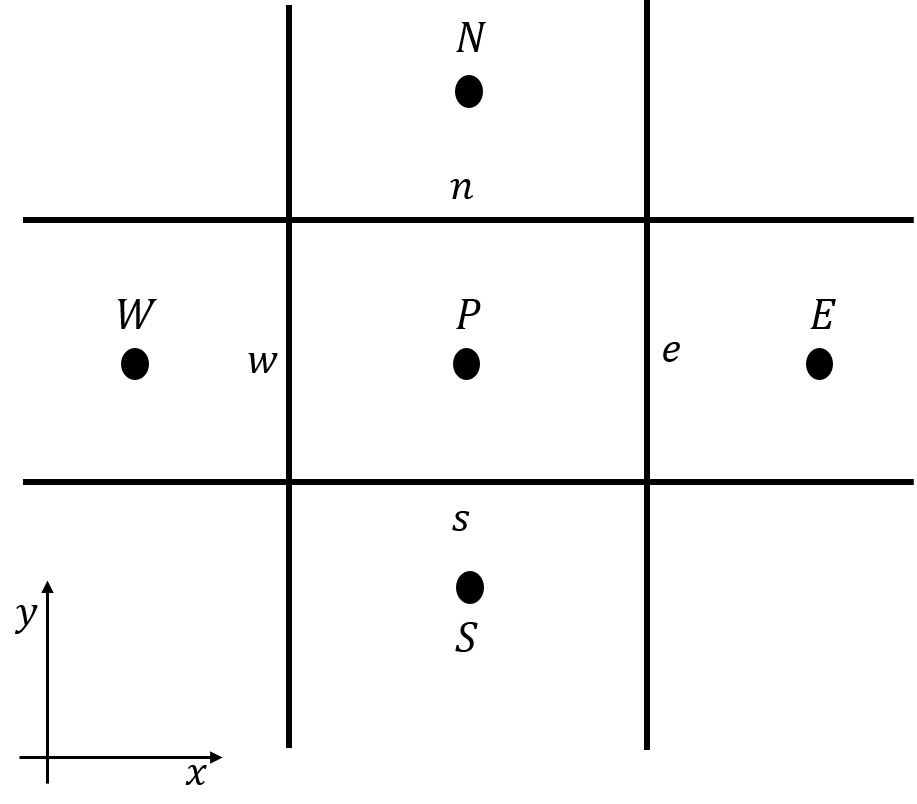
\includegraphics[width=0.75\textwidth]{ch2_litsurvey/Figures/2ddomainwaxisneigh.png}
        \caption{$2D$ control volume around a node $P$.}
        \label{fig:2dd}
    \end{subfigure}
    \caption{Control volume around a node $P$ in (a) $1D$ and (b) $2D$.}
\end{figure}
For instance, on a $1D$ domain (see figure~\ref{fig:1dd}) the discretized form of the convective term is
\begin{equation}
\sum_{\partial \Omega}\dot{m}_f u_j = (\dot{m}u)_e + (\dot{m}u)_w.
\end{equation}
and on a $2$D domain (see figure~\ref{fig:2dd}) the discretized form of the convective term is
\begin{equation}
\sum_{\partial \Omega}\dot{m}_f u_j = (\dot{m}u_j)_e + (\dot{m}u_j)_w + (\dot{m}u_j)_n + (\dot{m}u_j)_s.
\end{equation}
Here $e$,$w$,$n$ and $s$ represent the east, west, north and south face of the CV respectively and $u$ and $v$ are the horizontal and vertical components of velocity. The velocity at the face is reconstructed from the upwind direction which is determined based on the direction of mass flux at each face. For example, for the face $e$, let the neighboring node be $E$. The direction is found as follows. First compute the mass flux across the face, $\dot{m}_e$
\begin{equation*}
\dot{m}_e = \frac{1}{2}\rho (u_{i,P} + u_{i,E})n_i.
\end{equation*}
Define two temporary quantities,
\begin{align*}
\dot{m}_P = \frac{1}{2}(\dot{m}_e + |\dot{m}_e|), \\
\dot{m}_E = \frac{1}{2}(\dot{m}_e - |\dot{m}_e|).
\end{align*}
The upwind direction can then be found as,
\begin{align*}
dir_P = \left\lfloor \frac{\dot{m}_P}{|\dot{m}_e|}\right\rceil, \\
dir_E = \left\lfloor \frac{\dot{m}_E}{|\dot{m}_e|}\right\rceil.
\end{align*}
\noindent Here $ \left\lfloor\right\rceil$ represent rounding to the nearest integer. 
%Clearly, if the flow is from $P$ towards $E$, $\dot{m}_e$ is positive and $dir_P$ becomes $1$ while $dir_E$ becomes zero and vice versa. 
Finally, the velocity at the face $e$ can be found as
\begin{equation}
u_{j,e} = (dir_P) u_{j,P} + (dir_E) u_{j,E}.
\end{equation}
This gives a first order upwind approximation which as seen in section~\ref{sec:ch2disceqnphi} is not very accurate. The velocities at the nodes, $u_{i,P}$ and $u_{i,E}$ can be reconstructed at the face $e$ to obtain a second order upwind scheme. This option is available to the user. SU2 also has different slope limiters to maintain monotonicity of the upwind scheme. The effect of using a slope limiter was also shown in section~\ref{sec:ch2disceqnphi}.


\subsection{Time integration: Steady state problems}\label{sssec:timediscr}
Steady state problems are solved using a pseudo unsteady method. Instead of using an iterative algorithm the solution is marched in time. For steady state problems, the time integration is done using an implicit Euler scheme. Let the solution at a node $P$ at time $t^{n+1}$ be $U_i^{n+1}$. Using an implicit Euler scheme on equation~\ref{eq:fvmeqn},
\begin{equation}
\int_{\Omega}\frac{\partial U^{n+1}_P}{\partial t}d\Omega +R_P(U^{n+1}) + F^{p,n}_P \approx 
\frac{\partial U^{n+1}_P}{\partial t} |\Omega|_P + R_P(U^{n+1}) + F^{p,n}_P.
\end{equation}

A backward Euler time integration scheme is used to discretize the time derivative. The final discretized equation using the procedure outlined in section~\ref{sec:ch2disceqnphi}, can be written as
%Using the backward Euler implicit scheme on the time derivative,
%\begin{equation}
%\frac{U^{n+1}_P - U^n_P}{\Delta t^n_P}|\Omega| +R_P(U^{n+1})  = -F^{p,n}_P.
%\end{equation}
%Since the residual at time $t^{n+1}$ is also unknown, it is linearized about time $t^n$
%\begin{equation}
%R_P(U^{n+1})  = R_P(U^n) + \sum_{\mathcal{N}(P)}\frac{\partial R_P(U^n)}{\partial U_{\mathcal{N}(P)}}\Delta U^n_P + \mathcal{O}(\Delta t^2).
%\end{equation}
%This approximation is valid only when solving for a steady state solution. Thus, the final system of equations can be written as
%\begin{equation*}
%    \left( \frac{|\Omega|}{\Delta t_P^n}\delta_{ij}+\frac{\partial R_{P}(U^n_i)}{\partial U_{j}} \right) \Delta U_{j}^n=-R_P(U^n_j)-F_{P}^{p,n},
%\end{equation*}
%or
\begin{equation}
\boldsymbol{A}^n \Delta\mathbf{U}^n=\mathbf{B}^n.
\label{eq:momeqfinal}
\end{equation}
$\boldsymbol{A}^n$ is the matrix of coefficients at a time level $t^n$ like $\mathbf{a}_{P,i}^n$, 
\begin{align*}
\boldsymbol{A}^n = \begin{bmatrix}
\vdots & & \vdots  & & \vdots \\
 & \ddots & & \ddots  \\
\dots & & \mathbf{a}_{P,i}^n & & \dots\\
 & \ddots & & \ddots  \\
\vdots & & \vdots  & &\vdots
\end{bmatrix},
\end{align*}
$\Delta\mathbf{U}^n$ is the vector containing the update to the solution at all the nodes at a time level $t^n$ and $\mathbf{B}^n$ is the vector containing the residual and pressure contributions from all the nodes,
\begin{align*}
\Delta\mathbf{U}^n = \begin{pmatrix}
\vdots\\
\Delta U_{P,i}^n \\
\vdots
\end{pmatrix},
\qquad
\mathbf{B}^n = \begin{pmatrix}
\vdots \\
-R(U^{n}_{P,i})-F^{p}_i\\
\vdots
\end{pmatrix},
\quad
i=1,2,3.
\end{align*}
%Here  denotes the component of velocity.


%\begin{equation*}
%\boldsymbol{A}_{ij} = \left(\frac{|\Omega|}{\Delta t}\delta_{ij}+\frac{\partial R_{i}}{\partial U_{j}}\right),
%\end{equation*} 
%is the coefficient matrix and $\Delta U^n = U^{n+1}-U^n$ is the update to the solution at time $t^n$. 

A local time stepping scheme is used to accelerate the convergence as each cell advances at a suitable local time step. This local time step is calculated as the minimum of the time steps obtained from convective and viscous terms. The steady solution is obtained faster if larger time steps are used. Also, since time accuracy is not desired when running steady state simulations, the largest possible time step that does not cause the solution to diverge is chosen.
\begin{equation}
\Delta t = min(\Delta t_{conv}, \Delta t_{visc}),
\end{equation}
\begin{equation}
\Delta t_{conv} = CFL\frac{|\Omega|}{\lambda_{conv}}, \qquad
\Delta t_{visc} = CFL\frac{|\Omega|^2}{\lambda_{visc}}.
\end{equation}
where $CFL$ is a user defined value and
\begin{equation}
\lambda_{conv} = \sum_{f}|u_{i,f} n_{i,f}|\Delta S,
\end{equation}
is the sum of the magnitude of the projected face velocity across all the faces of the control volume surrounding a node and 
\begin{equation}
\lambda_{visc} = \sum_{f}C\frac{\mu_{tot}}{\rho}\Delta S^2,
\end{equation}
is the viscous spectral radius~\cite{SU22014}. Here $C$ is a constant and is set to $C=0.25$. In order to avoid the possibility of division by zero, the convective term is changed to 
\begin{equation}
\lambda_{conv} = \sum_{f}|(u_f + u_{ref}) \cdot \vec{n}_f|\Delta S,
\end{equation}
where $u_{ref}$ is a reference velocity. 
%Since the aim of the time integration is to reach a steady state solution, time accuracy is not important and the time step sizes are chosen to ensure fast convergence without causing divergence.
\subsubsection{SIMPLE}
As explained in chapter 2, the SIMPLE algorithm is used to calculate the velocity and pressure in an iterative manner. However, since a pseudo time stepping scheme is used for steady state problems, the time steps take the place of iterations. Thus starting from a time step $t^n$, the velocities and pressure at the next time step $t^{n+1}$ is found as follows. The momentum equations are first solved using the pressure, $p^{n}$ at time $t^n$ to give an estimated velocity field, $u_{i}^{\ast}$. 
\begin{equation}
u_{i}^{\ast} = u_{i}^{n} + \Delta u_{i},
\end{equation}
where $\Delta u_{i}$ is found from the solution of equation~\ref{eq:momeqfinal} as $\Delta u_{i} = \frac{\Delta U_{i}}{\rho}$. 
The estimated velocities and pressure are then corrected based on velocity and pressure corrections.
\begin{align}
u_i^{n+1} = u_i^{\ast} + u_i^{\prime},\label{eq:vcorr}\\
p^{n+1} = p^n + p^{\prime}.
\label{eq:pcorr}
\end{align}
The pressure and velocity corrections are found by solving a Poisson equation. The Poisson equation is derived based on the continuity equation and the momentum equations. This procedure is described in the following section.

\section{Continuity equation}
So far, only the momentum equations have been used to find an estimate of the velocity based on the existing pressure field. In order to correct the velocity estimations and the pressure, the continuity equation must be used to close the system of equations. However, since the continuity equation does not contain any pressure terms a new equation for pressure has to be obtained. This new equation for pressure is derived starting from the discrete form of the continuity equation for an incompressible flow 
\begin{equation}
    \int_{\Omega}\frac{\partial \rho u_i}{\partial x_i} \approx \sum_{\partial \Omega}\rho u_{f,i} n_{f,i}\Delta S = \sum_{\partial \Omega}\dot{m}_{f} = 0 ,
    \label{eq:mfeqn}
\end{equation}
where $u_f$ is the velocity at a face $f$, $\rho$ is the fluid density and $n_i$ is the unit outward face normal and $\Delta S$ is the area. Using a linear interpolation to find this face velocity on collocated grids leads to the well known checkerboard problem in the pressure as seen in the previous chapter and thus momentum interpolation techniques are used. Previously, the momentum interpolation proposed by Rhie and Chow~\cite{Rhie1983} was given with only a conceptual explanation. The same interpolation can also be seen as equivalent to writing a pseudo momentum equation at every face with the coefficients linearly interpolated from the momentum equations of the neighboring nodes~\cite{Moukalled}. Thus, in a sense the momentum interpolation mimics the staggered grid approach on collocated grids. This can also be interpreted as adding a third order derivative of the pressure to stabilize the oscillations in the pressure field~\cite{Ferziger2002}.
%\nomenclature[A]{$\dot{m}_f$}{Mass flux across a face $f$}

\subsection{Momentum interpolation of velocities}
In this section, equation~\ref{eq:RCorig} is derived using an alternative approach following Moukalled et al.~\cite{Moukalled} but adapted to the solution procedure used in SU2. The momentum equation in the $x$ direction for a node $P$ (see figure~\ref{fig:1dd}) can be written as
\begin{equation*}
\mathbf{a}_{P}^{n,u}\Delta u_{P}^n+\sum_{C \in \mathcal{N}(P)} \mathbf{a}_{C,u}^{n,u}\Delta u_{C}^n=-R(u_{P}^{n})- |\Omega|\left(\frac{\partial p^n}{\partial x}\right)_{P} 
\end{equation*}
where $\mathbf{a}_{P}^{n,u}$ is the coefficient of $u$, the velocity along the $x$ direction at the node $P$, $\mathbf{a}_{C}^{n,u}$ is the coefficient of the same velocity component at a node $C$ which is a neighbor of node $P$ ($C \in \mathcal{N}(P)$), $R(u_{P}^{n})$ is the residual computed explicitly and $|\Omega|$ is the volume of the control volume around node $P$. Here ${\mathcal{N}(P)}$ represents the neighbors the node $P$. Since the density is assumed to be constant, it is absorbed in to the coefficients $\mathbf{a}_{P}^{n,u}$ and $\mathbf{a}_{C}^{n,u}$.

The estimate of the velocity at a node $P$ for time level $n+1$ can be written as 
\begin{equation}
u_{P}^{\ast}=u_{P}^{n}+\Delta u_{P}^n=u_{P}^{n}-\frac{1}{\mathbf{a}_{P}^{n,u}}\left(R(u^{n}_{P})+\sum_{C \in \mathcal{N}(P)} \mathbf{a}_{C,u}^n\Delta u_{C}^n+|\Omega|\left(\frac{\partial p^n}{\partial x}\right)_{P} \right),
\end{equation}
Let $H(u^n_P)$ denote  
\begin{equation*}
H(u^n_P)=\frac{1}{\mathbf{a}_{P}^{n,u}}\left(R(u^{n}_{P})+\sum_{C \in \mathcal{N}(P)} \mathbf{a}_{C,u}^n\Delta u_{C}^n\right).
\end{equation*}
The velocity estimates at a node $P$ at time level $t^{n+1}$ can now be re-written as
\begin{equation}
u_{P}^{\ast} = u_{P}^n - H(u^n_P) - \frac{|\Omega|}{\mathbf{a}_{P}^{n,u}}\left(\frac{\partial p^n}{\partial x}\right)_{P}.
\label{eq:velatP}
\end{equation}
Since the pressure gradient used so far is only an estimate, the velocities found using this formula are also an estimate and do not yet satisfy the continuity equation and are thus denoted by $u^{\ast}_i$. 

%\begin{figure}[h]
%\centering
%\captionsetup{justification=centering}
% 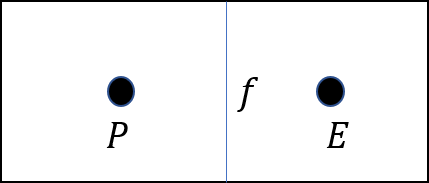
\includegraphics[width=0.2\textwidth]{ch3_su2eqn/figures/PEf_RCinterp.png}
%\caption{Nodes $P$ and $E$ across a face $f$.}
% \label{fig:pefrcinterp}
%\end{figure}
%\noindent
Consider another node $E$, which is a neighbor of node $P$ across the face $e$ in figure~\ref{fig:1dd}. The velocities at node $E$ can be written similar to equation~\ref{eq:velatP} as
\begin{equation}
u_{E}^{\ast} = u_{E}^n - H(u^n_E) -  \frac{|\Omega|}{\mathbf{a}_{E}^{n,u}}\left(\frac{\partial p^n}{\partial x}\right)_{E} .
\label{eq:velatE}
\end{equation}
Since the momentum interpolation technique mimics the staggered approach where velocities are stored on cell faces, hypothetically at the face $e$ between $P$ and $E$, the velocities, $u_{f,i}$ can be written as,
\begin{equation}
u_{e}^{\ast} = u_{e}^n - H(u^n_e) -  \frac{|\Omega|}{\mathbf{a}_{e}^{n,u}}\left(\frac{\partial p^n}{\partial x}\right)_{e} .
\label{eq:velatf}
\end{equation}

\noindent
The coefficients for the hypothetical momentum equation at the face $f$ are assumed to  be interpolated linearly from the neighboring nodes $P$ and $E$ as
\begin{equation}
H(u^n_e)=(\lambda_P H(u^n_P)+\lambda_E H(u^n_E)),
\label{eq:Beqn}
\end{equation}{}
\noindent where $\lambda_P$ and $\lambda_E$ are the weighting factors for the interpolation. Since a median dual grid is used for discretization, the faces are always midway between the two nodes. Thus, $\lambda_P = \lambda_E = 1/2$. Substituting for $H_{f,i}^n$, $H_{P,i}^n$ and $H_{E,i}^n$ in equation~\ref{eq:Beqn} from equations~\ref{eq:velatf}, \ref{eq:velatP} and \ref{eq:velatE} respectively and expanding the pressure source term from equation~\ref{eq:pressapprox}, the velocity at a face $f$ after the momentum equation is
\begin{align}
u_{e}^{\ast} &= u_{e}^n - \left(\lambda_P u_{P}^n + \lambda_E u_{E}^n \right) +\left(\lambda_P u_{P}^{\ast} + \lambda_E u_{E}^{\ast}\right) - \frac{|\Omega|_{f}}{\mathbf{a}_{e}^n}\left(\frac{\partial p^n}{\partial x}\right)_e \nonumber \\&+ \left(\lambda_P\frac{|\Omega|_{P}}{\mathbf{a}_{P}^n}\left(\frac{\partial p^n}{\partial x}\right)_{P} + \lambda_E\frac{|\Omega|_{E}}{\mathbf{a}_{E}^n}\left(\frac{\partial p^n}{\partial x}\right)_{E}\right) 
\label{eq:velatf*st1}
\end{align}
Let $\boldsymbol{D}_{P}^{n,u}$ denote
\begin{equation}
\boldsymbol{D}_{P}^{n,u} = \frac{|\Omega|}{\mathbf{a}_{P}^{n,u}}.
\label{eq:Dfeqn}
\end{equation}
Using the new notation, equation~\ref{eq:velatf*st1} can be written as
\begin{align}
u_{e}^{\ast} &= u_{e}^n - \left(\lambda_P u_{P}^n + \lambda_E u_{E}^n\right) +\left(\lambda_P u_{P}^{\ast} + \lambda_E u_{E}^{\ast}\right) - \boldsymbol{D}_{e}^{n,u}\left(\frac{\partial p^n}{\partial x_i}\right)_e \nonumber \\&+ \left(\lambda_P\boldsymbol{D}_{P}^{n,u}\left(\frac{\partial p^n}{\partial x}\right)_{P} + \lambda_E\boldsymbol{D}_{E}^{n,u}\left(\frac{\partial p^n}{\partial x}\right)_{E}\right).
\label{eq:velatf*st2}
\end{align}
The linear interpolation of the pressure gradient terms from nodes $P$ and $E$ are approximated as
\begin{align}
 \left(\lambda_P\boldsymbol{D}_{P}^{n,u}\left(\frac{\partial p^n}{\partial x}\right)_P + \lambda_E\boldsymbol{D}_{E}^{n,u}\left(\frac{\partial p^n}{\partial x}\right)_E\right) &=\overline{\boldsymbol{D}}_{e}^{n,u}\overline{\left(\frac{\partial p^n}{\partial x}\right)_e}.  \label{eq:pbarassump}
\end{align}
The terms under the over bar are linearly interpolated. This approximation is second order accurate~\cite{Moukalled}. Also the coefficient of the pressure gradient at the face is assumed to be the same as the linearly interpolated value i.e. 
\begin{align*}
\boldsymbol{D}_{e}^{n,u} &= \overline{\boldsymbol{D}}_{e}^{n,u}.
\end{align*}
Additionally, the linearly interpolated terms are written with an over bar as follows
\begin{align*}
(\lambda_P u_{P}^{\ast} + \lambda_E u_{E}^{\ast}) &= \overline{u}_{e}^{\ast}, \\
(\lambda_P u_{P}^{n} + \lambda_E u_{E}^{n}) &= \overline{u}_{e}^{n}.
\end{align*}
Equation~\ref{eq:velatf*st1} can now be written as
\begin{equation}
u_{e}^{\ast}=\overline{u}_{e}^{\ast}-\overline{\boldsymbol{D}}_{e}^{n,u}\left(\left(\frac{\partial p^n}{\partial x}\right)_{e}-\overline{\left(\frac{\partial p^n}{\partial x}\right)_{e}}\right) + \left(u_{e}^n - \overline{u}_{e}^n\right).
\label{eq:uvelatf*}
\end{equation}
Analogously, the $y$ and $z$ components of the velocity can be written as
\begin{align}
v_{e}^{\ast}&=\overline{v}_{e}^{\ast}-\overline{\boldsymbol{D}}_{e}^{n,v}\left(\left(\frac{\partial p^n}{\partial y}\right)_{e}-\overline{\left(\frac{\partial p^n}{\partial y}\right)_{e}}\right) + \left(v_{e}^n - \overline{v}_{e}^n\right).
\label{eq:vvelatf*}\\
w_{e}^{\ast}&=\overline{w}_{e}^{\ast}-\overline{\boldsymbol{D}}_{e}^{n,w}\left(\left(\frac{\partial p^n}{\partial z}\right)_{e}-\overline{\left(\frac{\partial p^n}{\partial z}\right)_{e}}\right) + \left(w_{e}^n - \overline{w}_{e}^n\right).
\label{eq:wvelatf*}
\end{align}

\subsubsection{Effect of pseudo time stepping}
Recall the expression for the face velocity based on the momentum interpolation in Eq. \ref{eq:uvelatf*}, 
\begin{equation*}
u_{e}^{\ast}=\overline{u}_{e}^{\ast}-\overline{\boldsymbol{D}}_{e}^{n,u}\left(\left(\frac{\partial p^n}{\partial x}\right)_{e}-\overline{\left(\frac{\partial p^n}{\partial x}\right)_{e}}\right) + \left(u_{e}^n - \overline{u}_{e}^n\right).
\end{equation*}
The first term on the RHS is the linearly interpolated velocity estimate and the second term is the difference of the pressure gradients. These two terms are identical to the original interpolation proposed by Rhie and Chow~\cite{Rhie1983}. However, the last term arises as a consequence of using the pseudo time stepping scheme in SU2. This term represents the difference between the corrected velocity at the face $u_e^n$ and the linearly interpolated value $\overline{u}_e^n$ from the previous time step. This difference is equivalent to the difference in pressure gradients from the previous time step. Thus, this term is zero at the start of the iteration and for every subsequent iteration, the difference between the two velocities, $u_e^n$ and $\overline{u}_e^n$ is carried over and added to the next iteration. Not considering this term can lead to oscillations in pressure at small time step sizes~\cite{Majumdar1988, Choi1999, Yu2002, Shen2012, Cubero2007, Bartholomew2018}.

In addition to this, the coefficient of the the pressure gradient contains the coefficients of the discretized momentum equations $\mathbf{a}_{e,u_i}^n$ which consists of contributions from time and spatial discretization as,
%\begin{equation*}
%\mathbf{a}_{f,i}^n = \frac{|\Omega|}{\Delta t_i^n}+\frac{\partial R_{i}(U^n)}{\partial U_{j}}.
%\end{equation*}
%Since the time step $\Delta t^n_i$ depends on the $CFL$ number, the interpolated velocity at the face and consequently the solution will also depend on the $CFL$ number. Denoting the contribution from the Jacobian and time discretization separately as 
\begin{equation*}
\mathbf{a}_{e,u_i}^n = \boldsymbol{a}_{e,u_i}^{t,n} + \boldsymbol{a}_{e,u_i}^{jac,n}.
\end{equation*}
Equation~\ref{eq:uvelatf*} can be rewritten as
\begin{equation*}
u_{e}^{\ast}=\overline{u_{e}^{\ast}}-\overline{\frac{|\Omega|}{\boldsymbol{a}_{e,u_i}^{t,n} + \boldsymbol{a}_{e,u_i}^{jac,n}}}\left(\left(\frac{\partial p^{n}}{\partial x}\right)_{e}-\overline{\left(\frac{\partial p^{n}}{\partial x}\right)_{e}}\right)+ \left(u_{e}^n - \overline{u}_{e}^n\right).
\end{equation*}
The contribution from the time discretization, $\boldsymbol{a}_{e,i}^{t,n}$ depends on the size of the time step $\Delta t$ which can be changed based on the user defined $CFL$ number. Thus, the final solution will be dependent on the external value of $CFL$ which is undesirable. This is also noted in Cubero and Fueyo~\cite{Cubero2007}. In order to eliminate this dependence the following approach can be adopted. A relaxation factor, $RC$, is introduced and multiplied to the time discretization contribution, $\alpha_t$. When this relaxation factor is set to zero, the solution is independent of $CFL$. It should be noted that this treatment is not derived analytically and can lead to convergence issues. The $RC$ factor can be changed based on convergence behavior.
\begin{equation*}
u_{e}^{\ast}=\overline{u_{e}^{\ast}}-\overline{\frac{|\Omega|}{RC\boldsymbol{a}_{e,u_i}^{t,n} + \boldsymbol{a}_{e,u_i}^{jac,n}}}\left(\left(\frac{\partial p^{n}}{\partial x_i}\right)_{e}-\overline{\left(\frac{\partial p^{n}}{\partial x_i}\right)_{e}}\right)+ \left(u_{e}^n - \overline{u}_{e}^n\right).
\end{equation*}

\subsection{Pressure correction equation}
To derive the pressure correction equation, first an equation for velocity corrections analogous to equation~\ref{eq:uvelatf*} is required. After applying the velocity and pressure corrections, the equation~\ref{eq:velatP} becomes
\begin{equation}
u_{P}^{n+1} = u_{P}^n - H(u^{n+1}_P) - \frac{|\Omega|}{\mathbf{a}_{P}^{n,u}}\left(\frac{\partial p}{\partial x}\right)^{n+1}_{P}.
\label{eq:velatPnp1}
\end{equation}
Subtracting equation~\ref{eq:velatPnp1} from equation~\ref{eq:velatP} gives an equation for velocity corrections as
\begin{equation}
u_{P}^{\prime} = - H(u^{\prime}_P) - \frac{|\Omega|}{\mathbf{a}_{P}^{n,u}}\left(\frac{\partial p^{\prime}}{\partial x}\right)_{P}.
\label{eq:uvelatP'}
\end{equation}
Following the same derivation steps outlined above to derive the equation for the velocity estimate at face $e$, $u_e^{\ast}$, a new equation for the velocity correction at a face $e$ between two nodes $P$ and $E$ (figure~\ref{fig:2dd}) can be derived as
\begin{equation}
u_{e}^{\prime}=\overline{u_{e}^{\prime}}-\overline{\boldsymbol{D}}_{e}^{n,u}\left(\left(\frac{\partial p^{\prime}}{\partial x}\right)_{e}-\overline{\left(\frac{\partial p^{\prime}}{\partial x}\right)}_{e}\right).
\label{eq:uvelatf'}
\end{equation}
Similarly, the equations for the velocity corrections in the other directions can be written as
\begin{align}
v_{e}^{\prime}&=\overline{v_{e}^{\prime}}-\overline{\boldsymbol{D}}_{e}^{n,v}\left(\left(\frac{\partial p^{\prime}}{\partial y}\right)_{e}-\overline{\left(\frac{\partial p^{\prime}}{\partial y}\right)}_{e}\right).
\label{eq:vvelatf'}\\
w_{e}^{\prime}&=\overline{w_{e}^{\prime}}-\overline{\boldsymbol{D}}_{e}^{n,w}\left(\left(\frac{\partial p^{\prime}}{\partial z}\right)_{e}-\overline{\left(\frac{\partial p^{\prime}}{\partial z}\right)}_{e}\right).
\label{eq:wvelatf'}
\end{align}
As before, the terms under the overbar are linearly interpolated. Before deriving the pressure correction equation, a new notation is introduced for the sake of simplicity.
\begin{equation}
\overline{S}_{f,x}^{n} = \overline{\boldsymbol{D}}_{f}^{n,u} n_{f,x}\Delta S,\quad \overline{S}_{f,y}^{n} = \overline{\boldsymbol{D}}_{f}^{n,v} n_{f,y}\Delta S \quad\text{and} \quad \overline{S}_{f,z}^{n} = \overline{\boldsymbol{D}}_{f}^{n,w} n_{f,z}\Delta S.
\end{equation}
Here $n_{f,i}$ is the outward facing unit normal of a face $f$, $\Delta S$ is the area of the face and $\overline{\boldsymbol{D}}_{f}^{n,u}, \overline{\boldsymbol{D}}_{f}^{n,v}$ and $\overline{\boldsymbol{D}}_{f}^{n,w}$ are the coefficients of the pressure gradient difference term in the velocity expressions (equations~\ref{eq:uvelatf'}, \ref{eq:vvelatf'} and \ref{eq:wvelatf'}) and is defined in equation~\ref{eq:Dfeqn}.

\noindent
Recall the continuity equation in discrete form equation~\ref{eq:mfeqn} 
\begin{equation*}
\sum_{f} \dot{m}_f = 0.
\end{equation*}
For a $1D$ control volume like the one shown in figure~\ref{fig:1dd}, the summation is over the faces $f=e,w$ and for a $2D$ control volume (figure~\ref{fig:2dd}, $f=e,w,n,s$.
Rewriting the discrete continuity equation in terms of estimated velocity and velocity corrections gives
\begin{equation}
\sum_{f}\dot{m}_{f}=\sum_{f}(\dot{m}_{f}^{\ast}+\dot{m}_{f}^{\prime})=0,
\end{equation}
where $\dot{m}^{\ast}_f$ and $\dot{m}^{\prime}_f$, the estimate and correction of the mass flux respectively, are computed as 
\begin{align*}
\dot{m}^{\ast}_f = \rho u_{f,i}^{\ast} n_{f,i} \Delta S,\\
\dot{m}^{\prime}_f = \rho u_{f,i}^{\prime} n_{f,i} \Delta S,
\end{align*}
Substituting for the velocity estimates (equations~\ref{eq:uvelatf*} to \ref{eq:wvelatf*}) and corrections (equations~\ref{eq:uvelatf'} to \ref{eq:wvelatf'}) in the equation~\ref{eq:mfeqn} gives,
\begin{equation}
\sum_{f}\rho\overline{u_{f,i}^{\prime}}n_{f,i}\Delta S-\rho\left(\left(\frac{\partial p^{\prime}}{\partial x_i}\right)_f-\overline{\left(\frac{\partial p^{\prime}}{\partial x_i}\right)_f}\right)\overline{S}_{f,i}^{n}=-\sum_{f}\dot{m}_{f}^{\ast}.
\end{equation}
Rearranging this equation by moving the linearly interpolated terms to the RHS gives
\begin{align}
-\sum_{f}\rho\overline{S}_{f,i}^{n}\left(\frac{\partial p^{\prime}}{\partial x_i}\right)_{f}=&-\sum_{f}\dot{m}_{f}^{\ast} \overbrace{-\sum_{f}\rho\overline{u_{f,i}^{\prime}}n_{f,i}\Delta S-\sum_{f}\rho\overline{S}_{f,i}^{n}\overline{\left(\frac{\partial p^{\prime}}{\partial x_i}\right)_{f}}}^{\text{neglected in SIMPLE}}.\label{eq:pcorrsu21} 
\end{align}
As outlined in section~\ref{sec:pcorrstag}, the terms under the over brace on the RHS of equation~\ref{eq:pcorrsu21} are neglected in the SIMPLE algorithm. The remaining term on the RHS of equation~\ref{eq:pcorrsu21} is the mass flux that is calculated using the estimated velocities. Thus, the pressure correction is
\begin{equation}
-\sum_{f}\rho\overline{S}_{f,i}^{n}\left(\frac{\partial p^{\prime}}{\partial x_i}\right)_{f}=-\sum_{f}\dot{m}_{f}^{\ast},
\label{eq:pcorreq}
\end{equation}
%or
%\begin{equation}
%-\sum_{f}\rho\overline{\boldsymbol{D}}_{f,i}\left(\frac{\partial p^{\prime}}{\partial x_i}\right)_{f} n_{f,i}\Delta S=-\sum_{f}\dot{m}_{f}^{\ast},
%\label{eq:pcorreq}
%\end{equation}
%where 
%\begin{equation}
%\overline{\boldsymbol{D}}_{f,i} = \overline{\frac{|\Omega|}{\mathbf{a}_{f,i}^n}}.
%\end{equation}
 Equation~\ref{eq:pcorreq} is a discretized Poisson equation for the pressure correction, $p^{\prime}$, with the uncorrected mass flux, $\sum_{f}\dot{m}_{f}^{\ast}$, being the source term. This equation has to be solved sequentially with the momentum equations. 

Since the pressure correction equation was derived starting from the continuity equation, the summation of the gradients of the pressure correction are also carried out on the same control volume. Across the control volume shown in figure~\ref{fig:1dd}, the summation will be over the faces $f=e,w$ and for the control volume in figure~\ref{fig:2dd}, the summation will be over the faces $f=e,w,n,s$. The discretized pressure correction gradient for face $e$ can be approximated as
\begin{equation*}
\left(\frac{\partial p^{\prime}}{\partial x_i}\right)_{f} \approx\frac{p_E^{\prime} - p_P^{\prime}}{d_{PE}}n_{f,i},
\end{equation*}
where $d_{PE}$ is the total distance between the nodes $P$ and $E$ across the face $f$ and $n_{f,i}$ is the outward unit normal of the face $f$. In order to find the coefficients of the nodal values of pressure correction, $p^{\prime}_P$, the term $\overline{S}_{f,i}^{n}$ must be calculated at each face $f$. $\overline{S}_{f,i}$ is calculated at a face $f$ using an over-relaxed approach~\cite{Moukalled}. The over-relaxed approach increases the contribution of the nodes $P$ and $E$ as the grid non-orthogonality increases. $\overline{S}_{f,i}^{n}$ is split into the orthogonal ($\overline{E}_{f,i}^{n}$) and non-orthogonal ($\overline{T}_{f,i}^{n}$) parts as
\begin{equation}
\overline{S}_{f,i}^{n} = \overline{E}_{f,i}^{n} + \overline{T}_{f,i}^{n}.
\end{equation}
The orthogonal contribution is treated implicitly and the non orthogonal contribution is neglected.  The pressure correction equation thus becomes
\begin{equation*}
-\sum_{f}\rho\overline{E}_{f,i}^{n}\left(\frac{\partial p^{\prime}}{\partial x_i}\right)_{f}=-\sum_{f}\dot{m}_{f}^{\ast},
\end{equation*}
The coefficients of the nodal values of $p^{\prime}$ calculated using the over-relaxed approach for the nodes $P$ and $E$ across the face $e$ is
\begin{equation}
a_{E}^{p^{\prime}} = (-\rho\Delta S)\frac{(\overline{\boldsymbol{D}}_{f}^{n,u}n_x)^2+(\overline{\boldsymbol{D}}_{f}^{n,v}n_y)^2+(\overline{\boldsymbol{D}}_{f}^{n,w}n_z)^2}{\overline{\boldsymbol{D}}_{f}^{n,u}d_{PE,x}+\overline{\boldsymbol{D}}_{f}^{n,v}d_{PE,y}+\overline{\boldsymbol{D}}_{f}^{n,w}d_{PE,z}},
\end{equation}
where $d_{PE,i}$ is the distance vector between nodes $P$ and $E$. Analogous to the discretization of the viscous terms in the scalar transport equation in section~\ref{sec:ch2disceqnphi}, the coefficients for all the nodal values can be assembled.  Thus, the pressure correction equation can be written as a system of linear equations as
\begin{equation}
a_P^{p^{\prime}} p_P^{\prime} + \sum_{C\in \mathcal{N}(P)}a_{C}^{p^{\prime}}p^{\prime}_C = -\sum_{f\in \mathcal{N}(P)} \dot{m}^{\ast}_f.
\end{equation}
The mass flux on the RHS is computed as the summation of the mass flux across the faces $f$ around the control volume of the node $P$. The system of equations for the nodal values of the pressure corrections $p^{\prime}_P$ can be solved using the linear solvers described in chapter 2. No under-relaxation is used for the Poisson solver. A multigrid method can be applied specifically for the Poisson problem to speed up the convergence, especially for unsteady problems.

\subsection{Pressure and velocity corrections}
Finally, based on the solution of the pressure correction equation, the pressure and velocities at a node $P$ can be corrected as
\begin{align}
&p_{P}^{n+1}=p_{P}^{\ast}+\alpha_{p}p^{\prime}, \label{eq:pcorrfinal}\\
&u_{P}^{n+1}=u_{P}^{\ast}+\boldsymbol{D}_{P}^{n,u}\left(\frac{\partial p^{\prime}}{\partial x}\right)_{P}, \nonumber\\
&v_{P}^{n+1}=v_{P}^{\ast}+\boldsymbol{D}_{P}^{n,v}\left(\frac{\partial p^{\prime}}{\partial y}\right)_{P},\label{eq:velcorrfinal}\\
&w_{P}^{n+1}=w_{P}^{\ast}+\boldsymbol{D}_{P}^{n,w}\left(\frac{\partial p^{\prime}}{\partial w}\right)_{P}\nonumber.
\end{align} 
%$D_P = \frac{|\Omega|}{diag(\boldsymbol{A})}\bigg|_P$ is the ratio of the volume of the element to the momentum equation coefficients at the node $P$ and 
$\alpha_p$ is the under-relaxation factor. There is no need to under-relax the velocity corrections since the pseudo time stepping method, used to solve the  momentum equations, acts as an under-relaxation for the velocities. The choice of the pressure under-relaxation will have an effect on the convergence of the system. 
As seen in chapter 2, the convergence of the SIMPLE algorithm can be accelerated if the pressure under-relaxation is set to
\begin{equation}
\alpha_p = 1+\frac{\sum_{f \in\mathcal{N}(P)} \mathbf{a}_{f,u_i}}{\mathbf{a}_{P,u_i}}.
\end{equation}
For a steady state solution, this factor can be simplified in terms of the velocity under-relaxation factor, $\alpha_v$, as
\begin{equation}
\alpha_p = 1 - \alpha_v,
\end{equation}
In order to find $\alpha_v$, recall the discretized momentum equation in the $x$ direction for a node $P$ is
\begin{equation*}
\mathbf{a}_{P}^{n,u}\Delta u_{P}^n+\sum_{C \in \mathcal{N}(P)} \mathbf{a}_{C}^{n,u}\Delta u_{C}^n=-R(u_{P}^{n})-|\Omega|\frac{\partial p^n}{\partial x}.
\end{equation*}
$\mathbf{a}_{P}^{n,u}$ contains contributions from the pseudo time stepping and the Jacobian and can be split as
\begin{equation}
\mathbf{a}_{P}^{n,u} = \boldsymbol{a}_{P}^{t,n} + \boldsymbol{a}_{P}^{jac,n},
\label{eq:urstart1}
\end{equation}
where $\boldsymbol{a}_{P}^{t,n}$ is the pseudo time stepping contribution and $\boldsymbol{a}_{P}^{jac,n}$ is the contribution from the Jacobian. Comparing to a typical under-relaxed equation of the form 
\begin{equation*}
\frac{\boldsymbol{a}_{P,u_i}^{jac,n}}{\alpha_v}\Delta u_{P,i}^n+\sum_{C \in \mathcal{N}(P)} \mathbf{a}_{C,u_i}^n\Delta u_{C,i}^n=-R(u_{P,i}^{n})-F_{P,i}^{p,n},
\end{equation*}
the under-relaxation factor in the pseudo time stepping scheme is
\begin{equation}
\alpha_v = \frac{\boldsymbol{a}_{P,u_i}^{jac,n}}{\boldsymbol{a}_{P,u_i}^{t,n} + \boldsymbol{a}_{P,u_i}^{jac,n}}.
\end{equation}
Thus, the optimum value of the pressure under-relaxation is
\begin{equation}
\alpha_p = 1 - \alpha_v = \frac{\boldsymbol{a}_{P,u_i}^{t,n}}{\boldsymbol{a}_{P,u_i}^{t,n} + \boldsymbol{a}_{P,u_i}^{jac,n}}.
\end{equation}


\section{Boundary conditions}

The control volume formed around interior nodes in the vertex based approach is shown in figure~\ref{fig:dualcell}. The node lies in the center of the control volume. However, because of the vertex based approach, the control volumes around the boundary nodes are different. The node lies on the face of the control volume at the physical boundary as shown in figure~\ref{fig:bddualcell}
\begin{figure}[h]
    \centering
    \captionsetup{justification=centering}
    \begin{subfigure}[b]{0.45\textwidth}
    \centering
    \captionsetup{justification=centering}
        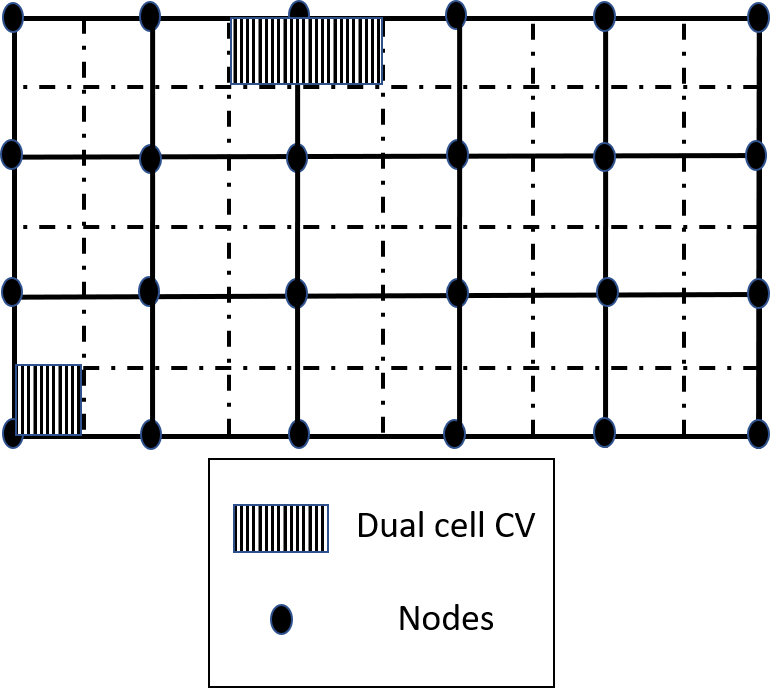
\includegraphics[width=.75\textwidth]{ch3_su2eqn/figures/boundary_dual_cell_nodes.png}
        \caption{Dual cell CV at boundaries.}
        \label{fig:bddualcell}
    \end{subfigure}
    ~ %add desired spacing between images, e. g. ~, \quad, \qquad, \hfill etc. 
      %(or a blank line to force the subfigure onto a new line)
    \begin{subfigure}[b]{0.45\textwidth}
    \centering
    \captionsetup{justification=centering}
        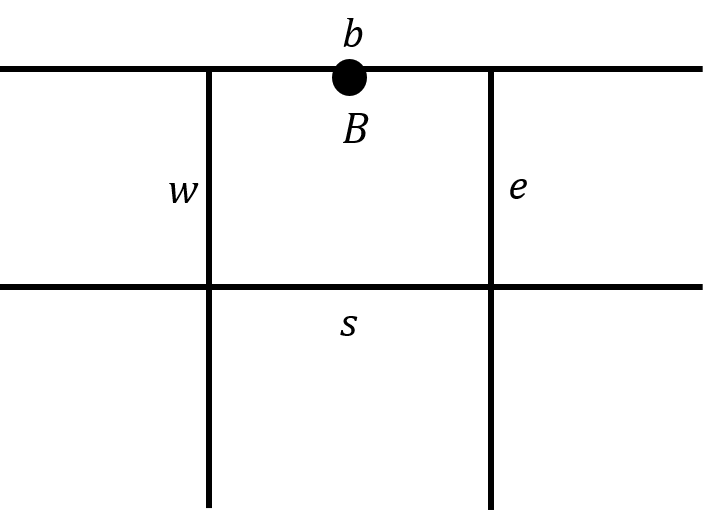
\includegraphics[width=0.75\textwidth]{ch3_su2eqn/figures/boundary_2ddomain.png}
        \caption{Boundary CV discretization.}
        \label{fig:bd2dd}
    \end{subfigure}
    \caption{Control Volume around boundary nodes.}
\end{figure}
While the discretization for the interior faces proceeds as described earlier, the discretization for the boundary face will be presented in this section. Since the boundary node ($B$) is directly on the boundary face ($b$) (figure~\ref{fig:bd2dd}), there is no need to use the momentum interpolation to find the velocity at the face, i.e. for any quantity $\phi$
\begin{equation}
\phi_b = \phi_B.
\end{equation}

The boundary conditions available are free slip wall, no slip wall, velocity inlet, pressure outlet and symmetry boundaries. The application of each of these boundary conditions for the momentum equations, mass flux computation and pressure correction equation is described below.
\subsection{Momentum equations}
\begin{enumerate}
    \item Slip wall: This boundary condition specifies a zero normal flux across the boundary (e.g. inviscid wall). For the momentum equations, this is applied as a weak boundary condition with zero flux across the face. The mass flux across the face is also set to zero.
\begin{equation}
\dot{m}_b = 0.
\end{equation}
    \item Wall (no-slip): This is a strong boundary condition and is generally used to impose a no slip condition on the velocities at the wall. Since the discretization is vertex-based the boundary node lies on boundary face and thus the velocity boundary condition can be enforced as a Dirichlet boundary condition. The mass flux across the face is set to zero and the velocity at the wall is set to zero or to the specified wall velocity ($u_{wall}$).
\begin{equation}
\dot{m}_b = 0, \quad u_b = u_{wall}.
\end{equation}
    \item Inlet: For a prescribed velocity ($u_{in}$) at the inlet, the velocity is imposed as a Dirichlet boundary condition similar to the wall boundary. However, the mass flux is not zero but can be easily computed based on the specified velocity $u_{in}$.
\begin{equation}
\dot{m}_b = \rho u_{i,in} n_i \Delta S_{b}, \quad u_b = u_{in}.
\end{equation}
    \item Outlet: For a specified pressure outlet, a weak boundary condition is applied for the velocities at the outlet. Fully developed flow conditions are assumed at the outlet. Thus, the velocity gradient normal to the outlet surface is zero. Similarly, the mass flux across the face is also computed using the latest estimate of the velocity.
    \begin{equation}
\dot{m}_b = \rho u_{i,b}n_i\Delta S_{b}.
\end{equation}
    \item Symmetry: A symmetry boundary does not only imply a zero flux across the face but also a reflection of the solution state across the boundary face. Consequently, a reflected state of the current state is computed and a Neumann boundary condition is applied. The mass flux across the face is set to zero.
    \item Far-field: Far-field boundaries are typically used in external flow simulations to denote the free-stream conditions. This is treated as an inlet-outlet type boundary where a Dirichlet condition is used for incoming flow and a Neumann boundary for outgoing flow based on the nature of the flux at the boundary face. The mass flux at the far-field face is computed as 
\begin{equation}
\dot{m}_b = \rho u_{i,b}n_i\Delta S_{b}.
\end{equation}
Depending on the sign of the mass flux, this face is treated as an inlet ($\dot{m}_b < 0$) or an outlet ($\dot{m}_b>0$). Implementation of these two conditions are similar to the inlet and outlet boundary conditions.
    \item Periodic: The periodic pair of elements are treated as an internal element by exchanging the flux across the interface. The solution is only computed for the donor node and is transformed back to the receiver node.
\end{enumerate}{}

\subsection{Pressure correction equations}
If the pressure at a particular boundary is unknown (Euler wall, Wall, Inlet, Symmetry) it is treated as a Neumann boundary and the value of the pressure is updated based on the pressure correction. However, if the value of the pressure is specified (Outlet with a specified pressure), the value of the pressure is fixed and the pressure correction is set to zero as a Dirichlet boundary condition.

%\subsection{Turbulence modeling}

%\textcolor{red}{[***May be it better to just mention the turbulence models within a paragraph***]}

%SU2 currently supports two RANS models - the Spalart-Allmaras(S-A) and the Mean Shear Stress Transport (SST) model are linked to the solver. 

%\nomenclature[A]{$C_d$}{Drag coefficient}
%\nomenclature[A]{$P$}{Pressure}
%\nomenclature[A]{$\vec{n}$}{Normal vector}
%\nomenclature[A]{$C_f$}{Skin friction coefficient}
%Here it is assumed $U_{f}^{n}=1/2(U_{P}^{n}+U_{E}^{n})$. This assumption is not valid at every time step and requires further attention. For now, the solution from the momentum equation is only an estimate which will be corrected based on the equation to be derived soon and at convergance when velocity field obeys both continuity and momentum equations, the assumption becomes valid and neglecting the term may be justified. However, this is a workaround and further attention is required

\section{Unsteady problems: Dual time stepping}
Unsteady problems are solved with a dual time stepping scheme. The unsteady problem is converted to a steady state problem within each time step which is solved as described previously. A pseudo transient term is added to equation~\ref{eq:fvmeqn} as
\begin{equation}
\int_{\Omega}\frac{\partial U}{\partial \tau}d\Omega + \int_{\Omega}\frac{\partial U}{\partial t}d\Omega + R(U) = -F^p \rightarrow \int_{\Omega}\frac{\partial U}{\partial \tau}d\Omega + R^{\ast}(U) = 0,
\label{eq:dualtime1}
\end{equation}
where $\tau$ is the pseudo time variable. The pseudo time term is discretized as explained in section~\ref{sssec:timediscr} and the unsteady time term is discretized by a backward Euler scheme. First and second order time integration schemes can be used for the unsteady term. For the first order discretization, $R^{\ast}(U)$ is
\begin{equation}
R^{\ast}(U) = \frac{U-U^n}{\Delta t}|\Omega| + R(U) + F^{p,n},
\end{equation}
and for second order,
\begin{equation}
R^{\ast}(U) = \frac{3U -4U^n +U^{n-1}}{2\Delta t}|\Omega| + R(U) + F^{p,n}.
\end{equation}
At the end of the pseudo-steady solution $U$ of equation~\ref{eq:dualtime1} becomes $U^{n+1}$.
\section{Moving grids}\label{sec:roteqn}
Recall the general form of equations in SU2 from equation~\ref{eq:generic} is 
\begin{equation*}
\frac{\partial U}{\partial t}  + \frac{\partial F^c_i}{\partial x_i}-\frac{\partial F^v_i}{\partial x_i}=Q \quad \text{in} \quad \Omega, \quad t>0.
\end{equation*}
\subsection{Arbitrary Lagrangian Eulerian method}
For the Arbitrary Lagrangian and Eulerian (ALE) formulation, the convective term is expressed as
\begin{equation}
F^c_i = \rho (u_i -u_{g,i})u_j,
\end{equation}
where $u_{g,i}$ is the grid velocity. The other terms remain the same. However, the computation of mass flux at the faces of control volumes must also account for the grid movement. Thus, the relative velocity at a face, $u_{rel,f}$, computed using the Rhie-Chow interpolation is 
\begin{equation}
u_{rel,f}^{\ast}=\overline{u_{f}}^{\ast} - \overline{u}_{f,g} -\overline{\boldsymbol{D}}^{n,u}_f\left(\left(\frac{\partial p^{\prime}}{\partial x}\right)_{f}-\overline{\left(\frac{\partial p^{\prime}}{\partial x}\right)_{f}}\right) + \left(u_{e}^n - \overline{u}_{e}^n\right).
\label{eq:velatfmov}
\end{equation}
Here $\overline{u}_{f,g}$ is the linearly interpolated grid velocity at the face $f$.
\subsubsection{Rotating reference frame}
For steady simulations, in a rotating reference frame with rotation rate $\Omega_i$, the grid velocity can be found as the cross product of the rotation rate vector and the radius vector.
\begin{equation}
u_{g,i} = \epsilon_{ijk} \Omega_i r_j\hat{e}_k.
\end{equation} 
The $\Omega_i$ is the vector of rotation rate about each of the axis, $r_j$ is the radius vector from the center of rotation, $\hat{e}_k$ is the unit coordinate vector and $\epsilon_{ijk}$ is the levi civita tensor. In addition to accounting for grid movement like described above an additional source term is added to the momentum equations
\begin{equation}
Q_{rot} = -\rho \epsilon_{ijk} \Omega_i u_j\hat{e}_k.
\end{equation}
This source term is the cross product of the rotation rate vector, $\Omega_i$, and the velocity vector, $u_j$.
\section{Turbulence modeling}
Turbulence modeling in SU2 is based on solving the Reynolds Averaged Navier Stokes (RANS) equations. As described in section~\ref{ssec:incomprans}, the most widely used approach is to use the Boussinesq hypothesis and write the Reynolds stresses in terms of mean flow gradients. This introduces a new unknown, the turbulent eddy viscosity, $\mu_t$. In order to close the system of RANS equations, equations for the turbulent eddy viscosity are solved. Eddy viscosity turbulence models implemented in SU2 are the Spalart-Allmaras (SA)~\cite{spalart1992one} and the Menter Shear Stress Transport (SST)~\cite{menter1994two} model. These are described in detail in this section.

\subsection{Spalart-Allmaras (SA)}
%\noindent
The SA eddy viscosity model is a one equation model and solves for a scalar variable $\tilde{\nu}$. This scalar is related to the eddy viscosity as
\begin{equation}
\mu_{tur} = \rho \tilde{\nu} f_{v1}.
\end{equation}
Here $\rho$ is the density and $f_{v1}$ is obtained from the turbulence model. Many different versions of the SA turbulence models are available~\cite{NASATMR}. The general form of the equation in all versions closely resembles the transport equation like equation~\ref{eq:genphi}. The standard SA model is
\begin{align}
\frac{\partial \tilde{\nu}}{\partial t} + u_j\frac{\partial \tilde{\nu}}{\partial x_j} = c_{b1}(1-f_{t2})\tilde{S}\tilde{\nu}-\left[c_{w1}f_w - \frac{c_{b1}}{\kappa^2}f_{t2} \right]\left(\frac{\tilde{\nu}}{d}\right)^2 \\+ \frac{1}{\sigma}\left[\frac{\partial}{\partial x_j}\left(\nu_{tot}\frac{\partial \tilde{\nu}}{\partial x_j}\right) + c_{b2}\frac{\partial \tilde{\nu}}{\partial x_i}\frac{\partial \tilde{\nu}}{\partial x_i}\right].\nonumber
\label{eq:saorig}
\end{align}
The definitions of the functions are
\begin{align}
f_{v1} &= \frac{\chi^3}{\chi^3 + c_{cv1}^2}, \nonumber \\
\chi &= \frac{\tilde{\nu}}{\nu},
\end{align}
where $\nu$ is the molecular kinematic viscosity. Additionally,
\begin{equation}
\tilde{S} = \Omega + \frac{\tilde{\nu}}{\kappa^2 d^2}f_{v2}.
\end{equation}
Here $\Omega$ is the magnitude of the vorticity, $d$ is the distance from the point to the nearest wall and
\begin{align}
f_{v2} = 1 - \frac{\chi}{1+\chi f_{v1}}.\nonumber 
\end{align}
$f_w$ is computed as
\begin{align}
f_w &= g\left[\frac{1+c_{w3}^6}{g^6+c_{w3}^6}\right]^{1/6},  \\
g = r + c_{w2}(r^6-r), &\quad r = \text{min}\left(\frac{\tilde{\nu}}{\tilde{S}\kappa^2d^2},10\right) \nonumber.
\end{align}
Finally, $f_{t2}$ is computed as
\begin{align}
f_{t2} = c_{t3}e^{-c_{t4}\chi^2} \nonumber.
\end{align}
The model constants are
\begin{align}
c_{b1} = 0.1355, \quad \sigma=2/3, \quad c_{b2} = 0.622, \nonumber \\
\kappa = 0.41, \quad c_{w2} = 0.3, \quad c_{v1} = 7.1, \\
c_{t3} = 1.2, \quad c_{t4} = 0.5, c_{w1} = \frac{c_{b1}}{\kappa^2} + \frac{1+c_{b2}}{\sigma}. \nonumber
\end{align}
The most widely used version of SA however ignores the trip term $f_{t2}$. This is referred to as the "no trip term" version of the SA turbulence model and is also used in SU2. In this variation the constant $c_{t3}$ is set to zero. The no trip SA turbulence model can now be written in the general form of equation~\ref{eq:generic} as 
\begin{equation*}
\frac{\partial U}{\partial t}  + \frac{\partial F^c_i}{\partial x_i}-\frac{\partial F^v_i}{\partial x_i}=Q \quad \text{in} \quad \Omega, \quad t>0,
\end{equation*}
where
\begin{align}
    U= \Tilde{\nu}, \qquad
    F^c_i = u_i \Tilde{\nu}, \qquad
    F^v_i = \frac{(\nu + \Tilde{\nu})}{\sigma}\frac{\partial \Tilde{\nu}}{\partial x_i} \nonumber, \\
    Q =  c_{b1}\Tilde{S}\Tilde{\nu} -c_{w1}f_w\big(\frac{\Tilde{\nu}}{d_S} \big)^2 + \frac{c_{b2}}{\sigma}\bigg|\frac{\partial \Tilde{\nu}}{\partial x_i}\bigg|^2.
    \label{eq:SAmodel}
\end{align}{}

\subsubsection{Discretization}
Since the turbulence model equation resembles the general scalar transport equation~\ref{eq:genphi}, the discretization is carried out as described in section~\ref{sec:ch2disceqnphi}. Since equation~\ref{eq:SAmodel} is solved sequentially after the momentum and pressure correction equations, the previously solved velocity field is used and the advective term, $F^c_i$ is discretized using an upwind scheme. The viscous term, $F^v_i$, is discretized using a central difference scheme. The source term is discretized using the midpoint integration rule where the gradients are computed with Green-Gauss theorem or the Least Squares method. 

\subsubsection{Boundary conditions}
The most important boundary conditions for the turbulence models are at the walls and far-field boundaries. The boundary condition for the SA turbulence model at the far-field boundaries is
\begin{equation}
\tilde{\nu}_{\infty} = 3 \nu_{\infty}\quad \text{to}\quad 5\nu_{\infty}, 
\end{equation}
and on solid walls 
\begin{equation}
\tilde{\nu} = 0.
\end{equation}
\subsection{Menter Shear Stress Transport (SST)}
The Menter Shear Stress Transport equation~\cite{menter1994two} is a two equation model for finding the turbulent eddy viscosity. The two equations solve for the turbulent kinetic energy, $k$ and specific dissipation rate, $\omega$. This formulation combines two popular two equation models - the $k$-$\omega$ turbulence model~\cite{wilcox1988komega,wilcox2008komega} and the $k$-$\epsilon$ turbulence model~\cite{launder1974kepsilon,jones1972kepsilon} with an additional correction for adverse pressure gradients. The $k$-$\omega$ formulation is used in the inner parts of the boundary layer and $k$-$\epsilon$ formulation in the remaining parts of the flow field. 
The two equations are
\begin{equation}
\frac{\partial \rho k}{\partial t} + \frac{\partial \rho u_j k}{\partial x_j} = P - \beta^* \rho\omega k + \frac{\partial}{\partial x_j}\left((\mu + \sigma_k \mu_t)\frac{\partial k}{\partial x_j} \right),
\label{eq:keqn}
\end{equation}
and
\begin{align}
\frac{\partial \rho\omega}{\partial t} + u_j\frac{\partial \rho u_j \omega}{\partial x_j} = \frac{\partial}{\partial x_j}\left((\mu + \sigma_k \mu_t)\frac{\partial \omega}{\partial x_j} \right) + \frac{\gamma}{\nu_t}P \\ -\beta \rho \omega^2 + 2(1-F_1)\frac{\rho\sigma}{\omega}{\frac{\partial k}{\partial x_i}}{\frac{\partial \omega}{\partial x_i}}.
\label{eq:omeqn}
\end{align}
Here $P$ is the production term given by
\begin{equation}
P = \tau_{ij} \frac{\partial u_i}{\partial x_j}.
\end{equation}
where $\tau_{ij}$ is the viscous stress tensor (equation~\ref{eq:viscstress}). The turbulent eddy viscosity is computed as
\begin{equation}
    \mu_t = \frac{\rho a_1 k}{\text{max}(a_1 \omega, \Omega F_2)},
    \label{eq:kweddyvisc}
\end{equation}{}
where $\rho$ is density, $\Omega$ is the vorticity magnitude, $\Omega = \sqrt{2W_{ij}W_{ij}}$ with 
\begin{equation*}
    W_{ij} = \frac{1}{2}\left(\frac{\partial u_i}{\partial x_j} - \frac{\partial u_j}{\partial x_i} \right).
\end{equation*}{} 
Every constant in the model is a blend of inner and outer value, blended as
\begin{equation*}
    \phi = \phi_1 F_1 + (1 - F_1)\phi_2,
\end{equation*}
where $\phi$ represents any of the constants defined in equation~\ref{eq:kwconst}. The blending functions are computed as
\begin{align*}
    &F_1 = tanh(arg_1 ^4), \\
    &arg_1 = min\Bigg[max\bigg(\frac{\sqrt{k}}{\beta^* \omega d}, \frac{500\nu}{d^2 \omega}\bigg), 
                     \frac{4\rho\sigma_{\omega_2} k}{CD_{k\omega}d^2}\Bigg], \\
    &CD_{k\omega} = max\bigg(2\sigma_{\omega_2}\frac{1}{\omega}\frac{\partial k}{\partial x_j}\frac{\partial \omega}{\partial x_j} ,10^{-20} \bigg), \\
    &F_2 = tanh(arg_2 ^4), \\
    &arg_2 = max\Bigg(2\frac{\sqrt{k}}{\beta^* \omega d}, \frac{500\nu}{d^2 \omega}\Bigg),
\end{align*}
with $d$ being the distance of any field point to the nearest wall.

The constants of the model are given by
\begin{align}{}
a_1 = 0.31, \quad \kappa = 0.41, \quad  \beta^* = 0.09,  \nonumber\\
\sigma_{k_1} = 0.85, \quad \sigma_{\omega_1} = 0.5, \quad \beta_1 = 0.075, \nonumber\\
\sigma_{k_2} = 1.0, \quad \sigma_{\omega_2} = 0.856, \quad  \beta_2 = 0.0828, \nonumber\\
\gamma_1 = \frac{\beta_1}{\beta^*} - \frac{\sigma_{\omega_1}\kappa^2}{\sqrt{\beta^*}}, \quad \gamma_2 = \frac{\beta_2}{\beta^*} - \frac{\sigma_{\omega_2}\kappa^2}{\sqrt{\beta^*}} \label{eq:kwconst}.
\end{align}
Following the general form of the equations in equation~\ref{eq:generic}, the equations~\ref{eq:keqn} and \ref{eq:omeqn} can be written as
\begin{align}
    U=\begin{bmatrix}{}
    \rho k \\
    \rho\omega
    \end{bmatrix},
    F_i^c = \begin{bmatrix}{}
    \rho u_i k \\
    \rho u_i \omega
    \end{bmatrix},
    F^v_i = \begin{bmatrix}{}
    (\mu + \sigma_k \mu_t) \frac{\partial k}{\partial x_i} \\
    (\mu + \sigma_{\omega} \mu_t) \frac{\partial \omega}{\partial x_i}
    \end{bmatrix} \nonumber \\ \nonumber\\
    Q = \begin{bmatrix}{}
    P - \beta^* \rho\omega k \\
    \frac{\gamma}{\nu_t}P - \beta \rho \omega^2 + 2(1-F_1)\frac{\rho\sigma}{\omega}{\frac{\partial k}{\partial x_i}}{\frac{\partial \omega}{\partial x_i}}
    \end{bmatrix}.
\end{align}{}

\subsubsection{Discretization}
Similar to the SA turbulence model, the advective term, $F^c_i$ is discretized using an upwind scheme, the viscous term, $F^v_i$, using a central scheme and the source term is discretized using the midpoint integration rule with the gradients computed using either the Green Gauss theorem or the Least Squares method. 

\subsubsection{Boundary conditions}
The boundary conditions at the far-field boundaries for the SST $k-\omega$ model are
\begin{align}
k_{\infty}  &= \frac{3}{2} V_{\infty}^2 TI^{2},\nonumber\\
\omega_{\infty} &= \frac{k_{\infty}}{\nu_{\infty}\frac{\mu_t}{\mu_{lam}}}.
\end{align}
Here $\nu_{\infty}$ is the kinematic viscosity in the free stream, $V_{\infty}$ is the free stream velocity magnitude, $\rho$ is the density and $TI$ is the turbulent intensity. The ratio $\mu_t/\mu_{lam}$ and turbulent intensity $TI$ are specified as inputs. 
On solid walls, the boundary conditions are 
\begin{align}
k &= 0, \nonumber \\
\omega &= 10 \frac{6 \nu}{\beta_1(\Delta d)^2}.
\end{align}
$\Delta d$ is the first cell height and $\beta_1$ is a model constant defined earlier.


%%%%%%%%%%%%%%%%%%%%%%%%%%%%%%%%%%%%%%%%%%%

\bibliographystyle{dissertation}
\bibliography{ch3_su2eqn/su2ch3}


%\references{su2references}
